%%===========================================================%%
%%                                                           %%
%%                        BACKGROUNDS                        %%
%%                                                           %%
%%===========================================================%%

\chapter{Backgrounds}\label{chap:backgrounds}

\section{Sources of background}
\subsection{Non-exclusive background}\label{sec:nonExclBkgd}

%---------------------------
\begin{figure}[ht!]
\centering%
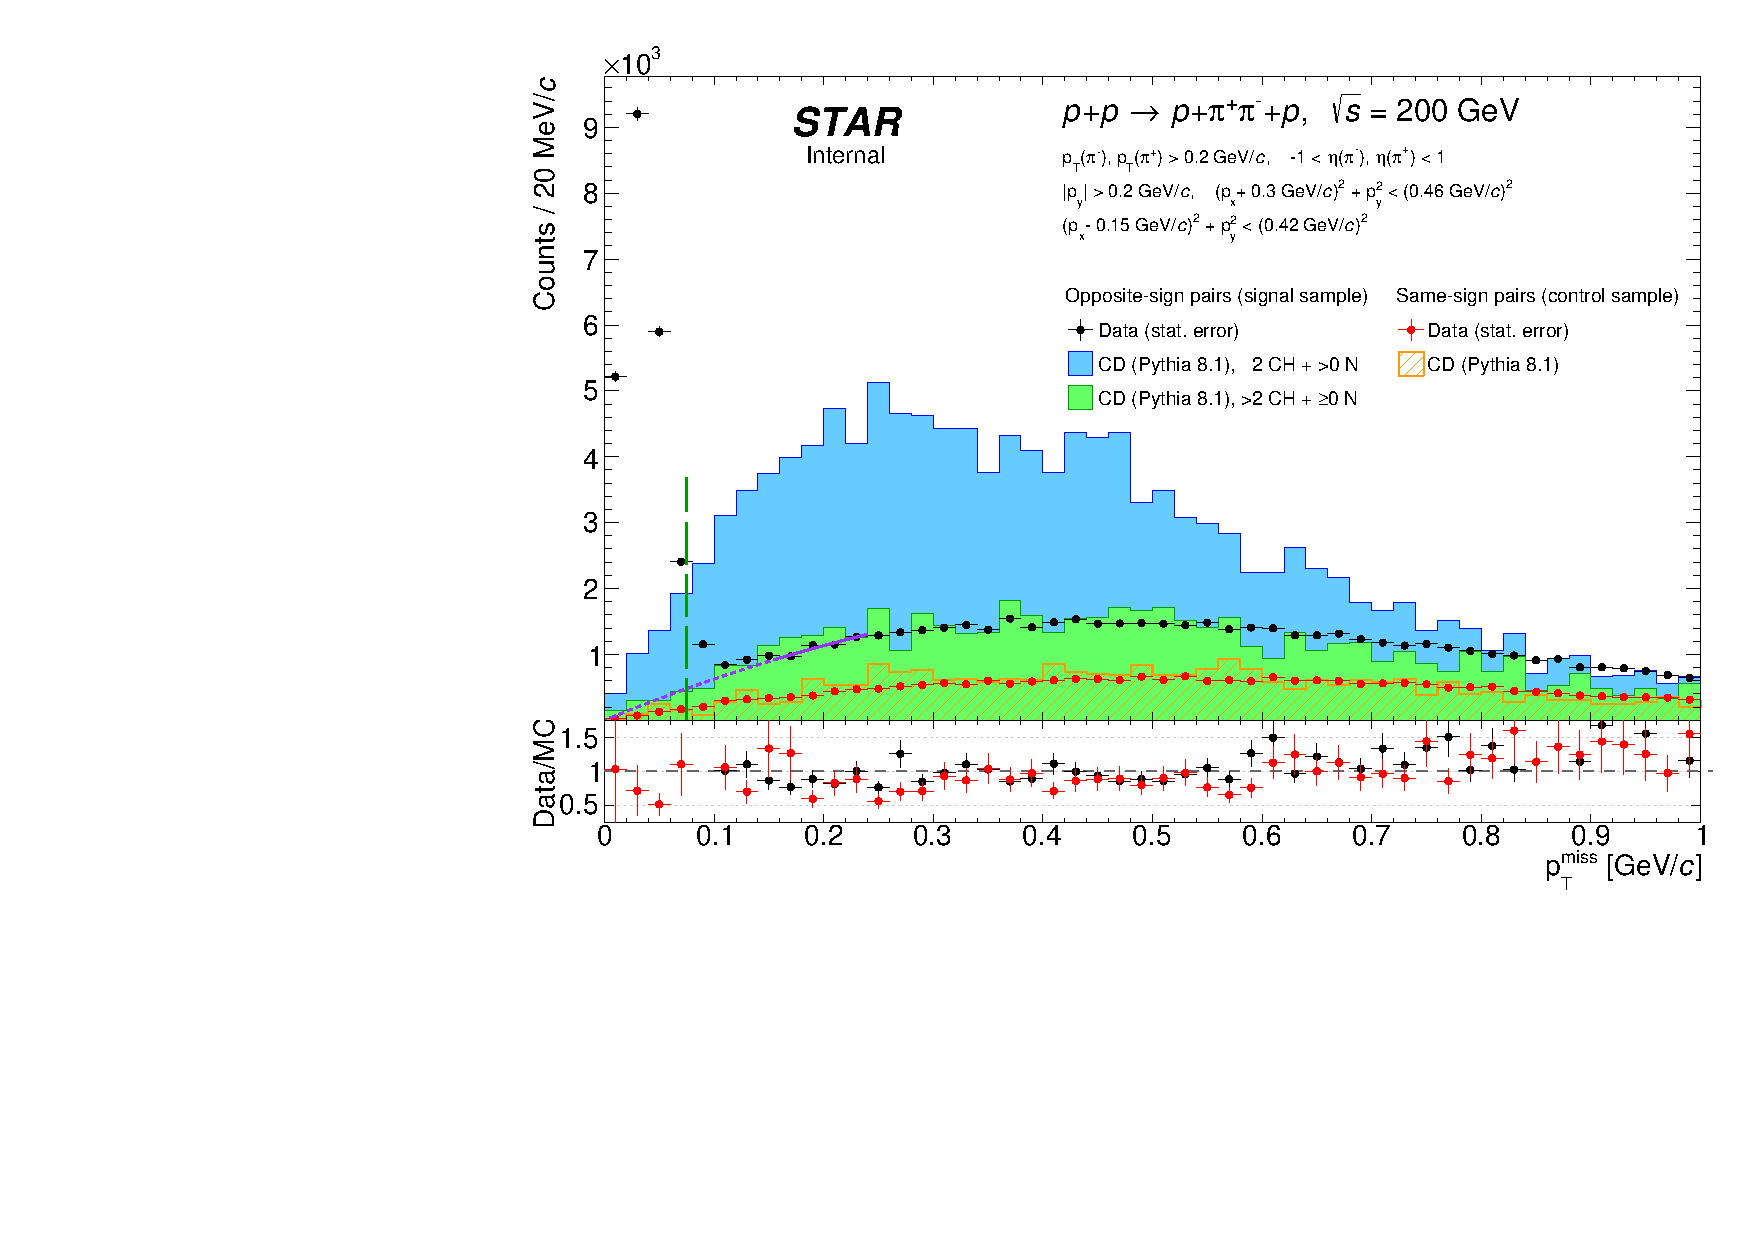
\includegraphics[width=0.65\linewidth,page=1]{graphics/backgrounds/Raw_MissingPtPid.pdf}%
\caption{Missing pT.}\label{fig:missingPtBkgd}%
\end{figure}
tutaj dodac szkice spodziewanego tla nieekskluzywnego
%---------------------------

\subsection{Exclusive background (particle misidentification)}\label{sec:exclBkgd}

%---------------------------
\begin{figure}[ht!]
\centering%
\parbox{0.4725\textwidth}{%
  \centering%
  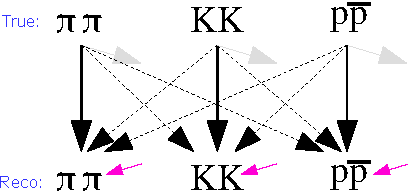
\includegraphics[width=\linewidth]{graphics/backgrounds/pid-crop2.pdf}\label{fig:misidentificationGraph}
}%
\quad%
\parbox{0.4725\textwidth}{%
    \caption[Graph illustrating the misidentification problem.]{Graph illustrating the misidentification problem - the origin of exclusive background in selected samples. Gray arrows represent event rejection due to failed PID selection (\ref{enum:CutPid}). Magenta arrows indicate non-exclusive backgrounds described in Sec.~\ref{sec:nonExclBkgd}. Solid black arrows represent successful identification, whereas dashed black lines show misidentification paths.}
}%

\end{figure}
%---------------------------


\begin{subequations}\label{eq:misidentificationEqs}
\begin{equation}
  N^{\pi\pi}_{R}~~=~~\begingroup\color{gray}\underbrace{\color{black}\epsilon^{\pi\pi}\cdot N^{\pi\pi}_{T}}_{\textrm{true pion pairs}}\endgroup~~ + ~~\begingroup\color{gray}\underbrace{\color{black}\lambda^{ KK\rightarrow \pi\pi}\cdot N^{KK}_{T}}_{\substack{\textrm{kaon pairs reconstructed} \\ \textrm{as pion pairs}}}\endgroup~~ + ~~\begingroup\color{gray}\underbrace{\color{black}\lambda^{p\bar{p} \rightarrow \pi\pi} \cdot N^{p\bar{p}}_{T}}_{\substack{\textrm{proton pairs reconstructed} \\ \textrm{as pion pairs}}}\endgroup~~ + ~~\textcolor{magenta}{N^{\pi\pi}_{bkgd}}
\end{equation}    
\begin{equation}
  N^{KK}_{R} ~= ~~\begingroup\color{gray}\underbrace{\color{black}\lambda^{ \pi\pi\rightarrow KK}\cdot N^{\pi\pi}_{T}}_{\substack{\textrm{pion pairs reconstructed} \\ \textrm{as kaon pairs}}}\endgroup~~ + ~~\begingroup\color{gray}\underbrace{\color{black}\epsilon^{KK}\cdot N^{KK}_{T}}_{\textrm{true kaon pairs}}\endgroup~~ + ~~\begingroup\color{gray}\underbrace{\color{black}\lambda^{p\bar{p} \rightarrow KK} \cdot N^{p\bar{p}}_{T}}_{\substack{\textrm{proton pairs reconstructed} \\ \textrm{as kaon pairs}}}\endgroup~~ + ~~\textcolor{magenta}{N^{KK}_{bkgd}}
\end{equation}
\begin{equation}\hspace*{-25pt}
  N^{p\bar{p}}_{R}~~~= ~~\begingroup\color{gray}\underbrace{\color{black}\lambda^{\pi\pi \rightarrow p\bar{p}} \cdot N^{\pi\pi}_{T}}_{\substack{\textrm{pion pairs reconstructed} \\ \textrm{as proton pairs}}}\endgroup~~ + ~~\begingroup\color{gray}\underbrace{\color{black}\lambda^{ KK\rightarrow p\bar{p}}\cdot N^{KK}_{T}}_{\substack{\textrm{kaon pairs reconstructed} \\ \textrm{as proton pairs}}}\endgroup~~ + ~~\begingroup\color{gray}\underbrace{\color{black}\epsilon^{p\bar{p}}\cdot N^{p\bar{p}}_{T}}_{\textrm{true proton pairs}}\endgroup~~ + ~~\textcolor{magenta}{N^{p\bar{p}}_{bkgd}}
\end{equation}
\end{subequations}

Eqs.~\eqref{eq:misidentificationEqs} can be written in the matrix form, as shown in Eq.~\eqref{eq:misidentificationMatrix}, from which it is straightforward to obtain final formula for unfolded number of events of given ID, Eq.~\eqref{eq:pidUnfoldingMatrix}:

\begin{tabulary}{\textwidth}{LCL}
\begin{equation}\label{eq:misidentificationMatrix}\hspace*{-15pt}
\Spvek{N^{\pi\pi}_{R}-\textcolor{magenta}{N^{\pi\pi}_{bkgd}};~;N^{KK}_{R}-\textcolor{magenta}{N^{KK}_{bkgd}};~;N^{p\bar{p}}_{R}-\textcolor{magenta}{N^{p\bar{p}}_{bkgd}}} =  \underbrace{\left[ \begin{array}{ccc}
\epsilon^{\pi\pi} & \lambda^{ KK\rightarrow \pi\pi} & \lambda^{p\bar{p} \rightarrow \pi\pi} \\
~ & ~ & ~\\
\lambda^{\pi\pi\rightarrow KK} & \epsilon^{KK} & \lambda^{ p\bar{p} \rightarrow KK}\\
~ & ~ & ~\\
\lambda^{\pi\pi\rightarrow p\bar{p}} & \lambda^{ KK\rightarrow p\bar{p}} & \epsilon^{p\bar{p}}
\end{array} \right]}_{\text{``mixing matrix''}~\Lambda}\Spvek{N^{\pi\pi}_{T};~;N^{KK}_{T};~;N^{p\bar{p}}_{T}}
\end{equation}&%
\vspace{40pt}$\rightarrow$\hspace{20pt}&
\begin{equation}\label{eq:pidUnfoldingMatrix}
\Spvek{N^{\pi\pi}_{T};~;N^{KK}_{T};~;N^{p\bar{p}}_{T}} = \Lambda^{-1}\Spvek{N^{\pi\pi}_{R}-\textcolor{magenta}{N^{\pi\pi}_{bkgd}};~;N^{KK}_{R}-\textcolor{magenta}{N^{KK}_{bkgd}};~;N^{p\bar{p}}_{R}-\textcolor{magenta}{N^{p\bar{p}}_{bkgd}}}
\end{equation}
\end{tabulary}


\section{Background and signal relative normalization}\label{sec:bkgdSignalNorm}

